% =====================================================================
%  Exercise Sheet Template  (compile with XeLaTeX or LuaLaTeX)
%  Layout: Part -> worked Example (numbered steps + dotted connectors)
%          -> Practice Questions (1 or 2 columns, optional visual models)
% =====================================================================
\documentclass{article}
\usepackage[margin=0.75in]{geometry}
\usepackage{xcolor}
\usepackage{amsmath}
\usepackage{amssymb}
\usepackage{fontspec}
\usepackage{tikz}
\usetikzlibrary{tikzmark, arrows.meta, positioning, decorations.pathreplacing, calc}
\usepackage{enumitem}
\usepackage{multicol}

% ---------------------------------------------------------------------
%  THEME & COLORS (Matching Base-10 3D Block Palette)
% ---------------------------------------------------------------------
\definecolor{bglight}{HTML}{FFFFFF}
\definecolor{textlight}{HTML}{000000}
\definecolor{subtext}{HTML}{666666}

% 3D Base-10 Block Colors
\definecolor{flatyellow}{HTML}{F3E222}
\definecolor{flatyellowtop}{HTML}{FFF066}
\definecolor{flatyellowside}{HTML}{C8B400}

\definecolor{rodpink}{HTML}{E64A85}
\definecolor{rodpinktop}{HTML}{FF80B3}
\definecolor{rodpinkside}{HTML}{B3245B}

\definecolor{unitblue}{HTML}{2A83CE}
\definecolor{unitbluetop}{HTML}{66B3FF}
\definecolor{unitblueside}{HTML}{1A538A}

\pagecolor{bglight}
\color{textlight}
\pagestyle{empty}

% ---------------------------------------------------------------------
%  BUILDING BLOCKS
% ---------------------------------------------------------------------

% Circled step number.  \stepnum{number}{node-name}
\newcommand{\stepnum}[2]{%
  \tikzmarknode{#2}{%
    \begin{tikzpicture}[baseline=(char.base)]
      \node[draw=textlight, circle, inner sep=1.5pt, font=\sffamily\small] (char) {#1};
    \end{tikzpicture}%
  }%
}

% Dotted connectors between consecutive step nodes.
\newcommand{\stepchain}[1]{%
  \begin{tikzpicture}[remember picture, overlay]
    \def\prevnode{}%
    \foreach \n in {#1} {%
      \ifx\prevnode\empty\else
        \draw[dotted, thick, textlight!60] (\prevnode.south) -- (\n.north);%
      \fi
      \xdef\prevnode{\n}%
    }%
  \end{tikzpicture}%
}

% Worked-example steps
\newenvironment{steps}{\begin{description}[leftmargin=2em]}{\end{description}}

% Practice questions
\newenvironment{questions}[1][1]{%
  \begin{enumerate}[label=\textbf{\arabic*.}, start=#1, itemsep=2em, leftmargin=2em]%
}{\end{enumerate}}

% Headings
\newcommand{\examplehead}[1]{{\Large \textbf{Example: #1}}\par\vspace{0.5em}}
\newcommand{\practicehead}[1]{%
  \vspace{1em}\noindent\textcolor{subtext!40}{\rule{\linewidth}{0.5pt}}\vspace{1.5em}\par
  {\Large \textbf{#1}}\par\vspace{1em}}

% Answer blanks
\newcommand{\blank}[1][1.5cm]{\underline{\hspace{#1}}}
\newcommand{\ans}[1]{{\color{subtext}#1}}

% ---------------------------------------------------------------------
%  3D BASE-10 BLOCK MACROS (Hundreds Flats, Tens Rods, Ones Units)
% ---------------------------------------------------------------------

% 3D Unit Cube (Ones)
\newcommand{\unitcube}[2]{%
  \begin{scope}[shift={(#1,#2)}]
    \draw[fill=unitblue, draw=black, line width=0.35pt] (0,0) rectangle (0.25,0.25);
    \draw[fill=unitbluetop, draw=black, line width=0.35pt] (0,0.25) -- (0.08,0.33) -- (0.33,0.33) -- (0.25,0.25) -- cycle;
    \draw[fill=unitblueside, draw=black, line width=0.35pt] (0.25,0) -- (0.33,0.08) -- (0.33,0.33) -- (0.25,0.25) -- cycle;
  \end{scope}%
}

% 3D Rod (Tens)
\newcommand{\tenrod}[2]{%
  \begin{scope}[shift={(#1,#2)}]
    \draw[fill=rodpink, draw=black, line width=0.35pt] (0,0) rectangle (0.25,2.5);
    \foreach \i in {1,...,9} {
      \draw[line width=0.2pt, black!80] (0,\i*0.25) -- (0.25,\i*0.25);
    }
    \draw[fill=rodpinktop, draw=black, line width=0.35pt] (0,2.5) -- (0.08,2.58) -- (0.33,2.58) -- (0.25,2.5) -- cycle;
    \draw[fill=rodpinkside, draw=black, line width=0.35pt] (0.25,0) -- (0.33,0.08) -- (0.33,2.58) -- (0.25,2.5) -- cycle;
    \foreach \i in {1,...,9} {
      \draw[line width=0.2pt, black!80] (0.25,\i*0.25) -- (0.33,\i*0.25+0.08);
    }
  \end{scope}%
}

% Single 3D Flat (Hundreds)
\newcommand{\hundredflat}[2]{%
  \begin{scope}[shift={(#1,#2)}]
    \draw[fill=flatyellow, draw=black, line width=0.35pt] (0,0) rectangle (2.5,2.5);
    \foreach \i in {1,...,9} {
      \draw[line width=0.2pt, black!70] (\i*0.25,0) -- (\i*0.25,2.5);
      \draw[line width=0.2pt, black!70] (0,\i*0.25) -- (2.5,\i*0.25);
    }
    \draw[fill=flatyellowtop, draw=black, line width=0.35pt] (0,2.5) -- (0.08,2.58) -- (2.58,2.58) -- (2.5,2.5) -- cycle;
    \foreach \i in {1,...,9} {
      \draw[line width=0.2pt, black!70] (\i*0.25,2.5) -- (\i*0.25+0.08,2.58);
    }
    \draw[fill=flatyellowside, draw=black, line width=0.35pt] (2.5,0) -- (2.58,0.08) -- (2.58,2.58) -- (2.5,2.5) -- cycle;
    \foreach \i in {1,...,9} {
      \draw[line width=0.2pt, black!70] (2.5,\i*0.25) -- (2.58,\i*0.25+0.08);
    }
  \end{scope}%
}

% Staggered Stack of 3D Flats
\newcommand{\flatstack}[3]{%
  \begin{scope}[shift={(#1,#2)}]
    \pgfmathsetmacro{\count}{#3}
    \foreach \s in {1,...,\count} {
      \pgfmathsetmacro{\dx}{(\count - \s) * -0.12}
      \pgfmathsetmacro{\dy}{(\count - \s) * 0.12}
      \hundredflat{\dx}{\dy}
    }
  \end{scope}%
}

% =====================================================================
\begin{document}
\sffamily

% ================= HEADER =================
\begin{center}
  {\Huge \bfseries Base-Ten Blocks \& Place Value} \\[0.4em]
  {\Large \textcolor{subtext}{Addition and Subtraction with Hundreds, Tens, and Ones}}
\end{center}
\vspace{1em}

% =====================================================================
%  PART 1 -- Reading 3D Base-10 Blocks
% =====================================================================
\section*{Part 1: Representing Numbers with 3D Blocks}

\examplehead{Find the total value of the blocks shown below}

\begin{steps}
  \item[\stepnum{1}{p1s1}] \textbf{Identify Hundreds (Yellow Flats), Tens (Pink Rods), and Ones (Blue Cubes)}\\[0.6em]
  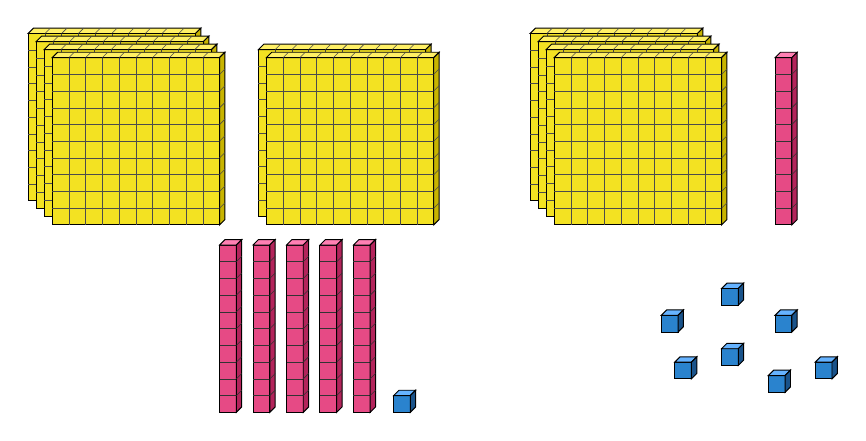
\begin{tikzpicture}[scale=0.85, transform shape]
    % Left Group: 4 Flats stack, 2 Flats stack, 5 Rods, 1 Unit
    \flatstack{0}{2.8}{4}
    \flatstack{3.2}{2.8}{2}
    
    \tenrod{2.5}{0}
    \tenrod{3.0}{0}
    \tenrod{3.5}{0}
    \tenrod{4.0}{0}
    \tenrod{4.5}{0}
    \unitcube{5.1}{0}

    % Right Group: 4 Flats stack + 1 Rod, 7 Units
    \flatstack{7.5}{2.8}{4}
    \tenrod{10.8}{2.8}

    \unitcube{9.1}{1.2}
    \unitcube{10.0}{1.6}
    \unitcube{10.8}{1.2}
    \unitcube{9.3}{0.5}
    \unitcube{10.0}{0.7}
    \unitcube{10.7}{0.3}
    \unitcube{11.4}{0.5}
  \end{tikzpicture}
  \vspace{0.6em}

  \item[\stepnum{2}{p1s2}] \textbf{Count each group}\\[0.2em]
  \begin{itemize}
    \item \textbf{Left side:} $6\text{ Hundreds} + 5\text{ Tens} + 1\text{ One} = 600 + 50 + 1 = 651$
    \item \textbf{Right side:} $4\text{ Hundreds} + 1\text{ Ten} + 7\text{ Ones} = 400 + 10 + 7 = 417$
  \end{itemize}
  \vspace{0.6em}

  \item[\stepnum{3}{p1s3}] \textbf{Find the total sum}\\[0.4em]
  \[ 651 + 417 = \mathbf{1068} \]
\end{steps}
\stepchain{p1s1,p1s2,p1s3}

\practicehead{Practice Questions}

\begin{questions}
  % Question 1: Reading 3D Blocks
  \item \textbf{Write the number represented by the blocks below:}

  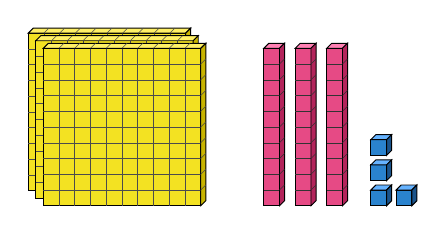
\begin{tikzpicture}[scale=0.8, transform shape]
    \flatstack{0}{0}{3}
    \tenrod{3.5}{0} \tenrod{4.0}{0} \tenrod{4.5}{0}
    \unitcube{5.2}{0} \unitcube{5.2}{0.4} \unitcube{5.2}{0.8} \unitcube{5.6}{0}
  \end{tikzpicture}

  \vspace{0.5em}
  $\blank\text{ Hundreds} + \blank\text{ Tens} + \blank\text{ Ones} = \blank$

  % Question 2: Addition with blocks
  \item \textbf{Find the sum of $235 + 124$ using place value blocks:}

  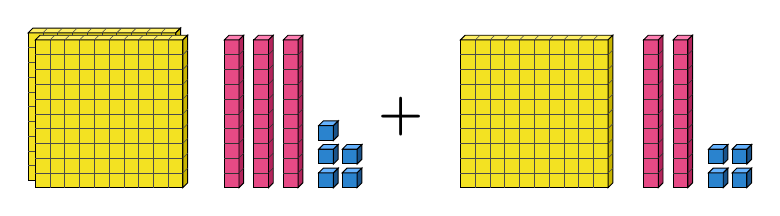
\begin{tikzpicture}[scale=0.75, transform shape]
    % 235
    \flatstack{0}{0}{2}
    \tenrod{3.2}{0} \tenrod{3.7}{0} \tenrod{4.2}{0}
    \unitcube{4.8}{0} \unitcube{4.8}{0.4} \unitcube{4.8}{0.8} \unitcube{5.2}{0} \unitcube{5.2}{0.4}

    \node[font=\Huge\bfseries] at (6.2,1.2) {+};

    % 124
    \hundredflat{7.2}{0}
    \tenrod{10.3}{0} \tenrod{10.8}{0}
    \unitcube{11.4}{0} \unitcube{11.4}{0.4} \unitcube{11.8}{0} \unitcube{11.8}{0.4}
  \end{tikzpicture}

  \vspace{0.6em}
  Total $= \blank\text{ Hundreds} + \blank\text{ Tens} + \blank\text{ Ones} = \blank$
\end{questions}

\pagebreak

% =====================================================================
%  PART 2 -- Base-10 Subtraction with 3D Blocks
% =====================================================================
\section*{Part 2: Base-10 Subtraction (Taking Away)}

\noindent\textbf{Example:} Solve \textbf{$345 - 123$} by crossing out blocks.
\vspace{0.8em}

\begin{steps}
  \item[\stepnum{1}{p2s1}] \textbf{Build the starting number ($345$)}\\[0.4em]
  Draw 3 Hundreds Flats, 4 Tens Rods, and 5 Ones Cubes.
  \vspace{0.4em}

  \item[\stepnum{2}{p2s2}] \textbf{Take away $123$ (1 Flat, 2 Rods, 3 Cubes)}\\[0.4em]
  Cross out the subtracted blocks with red lines:
  \\[0.6em]
  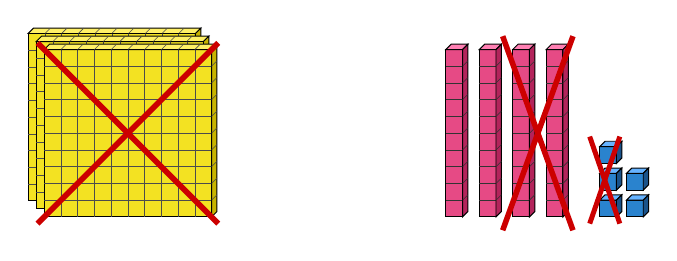
\begin{tikzpicture}[scale=0.85, transform shape]
    % 3 Hundreds (1 crossed out directly over the front flat)
    \flatstack{0}{0}{3}
    \draw[red!80!black, line width=2pt] (-0.1,-0.1) -- (2.6,2.6);
    \draw[red!80!black, line width=2pt] (-0.1,2.6) -- (2.6,-0.1);

    % 4 Tens (2 crossed out)
    \tenrod{6.0}{0} \tenrod{6.5}{0} \tenrod{7.0}{0} \tenrod{7.5}{0}
    \draw[red!80!black, line width=2pt] (6.85,-0.2) -- (7.9,2.7);
    \draw[red!80!black, line width=2pt] (6.85,2.7) -- (7.9,-0.2);

    % 5 Ones (3 crossed out)
    \unitcube{8.3}{0} \unitcube{8.3}{0.4} 
    \unitcube{8.3}{0.8} \unitcube{8.7}{0} \unitcube{8.7}{0.4}
    \draw[red!80!black, line width=1.8pt] (8.15,-0.1) -- (8.6,1.2);
    \draw[red!80!black, line width=1.8pt] (8.15,1.2) -- (8.6,-0.1);
  \end{tikzpicture}
  \vspace{0.6em}

  \item[\stepnum{3}{p2s3}] \textbf{Count remaining blocks}\\[0.2em]
  Remaining $= 2\text{ Hundreds}, 2\text{ Tens}, 2\text{ Ones}$ \\[0.2em]
  \[ 345 - 123 = \mathbf{222} \]
\end{steps}
\stepchain{p2s1,p2s2,p2s3}

\practicehead{Practice Questions}

\begin{questions}
  % Question 1: Subtraction by crossing out
  \item \textbf{Cross out blocks to calculate $246 - 114$:}

  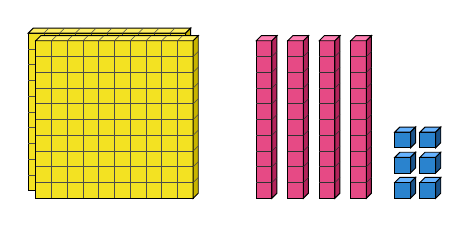
\begin{tikzpicture}[scale=0.8, transform shape]
    \flatstack{0}{0}{2}
    \tenrod{3.5}{0} \tenrod{4.0}{0} \tenrod{4.5}{0} \tenrod{5.0}{0}
    \unitcube{5.7}{0} \unitcube{5.7}{0.4} \unitcube{5.7}{0.8}
    \unitcube{6.1}{0} \unitcube{6.1}{0.4} \unitcube{6.1}{0.8}
  \end{tikzpicture}

  \vspace{0.6em}
  Remaining: $\blank\text{ Hundreds} + \blank\text{ Tens} + \blank\text{ Ones} = \blank$

  % Question 2: Regrouping Tens to Ones
  \item \textbf{Regrouping Tens to Ones: Calculate $132 - 115$}
  
  \textit{Hint: Trade 1 Pink Ten Rod for 10 Blue Unit Cubes first, then take away 5 ones.}

  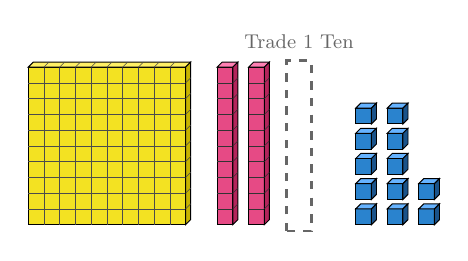
\begin{tikzpicture}[scale=0.8, transform shape]
    \hundredflat{0}{0}
    \tenrod{3.0}{0} \tenrod{3.5}{0}
    
    % Traded Rod space
    \draw[dashed, draw=subtext, line width=1pt] (4.1,-0.1) rectangle (4.5,2.6);
    \node[font=\small, text=subtext, align=center] at (4.3,2.9) {Trade 1 Ten};
    
    % 2 original ones + 10 traded ones
    \unitcube{5.2}{0} \unitcube{5.2}{0.4} \unitcube{5.2}{0.8} \unitcube{5.2}{1.2} \unitcube{5.2}{1.6}
    \unitcube{5.7}{0} \unitcube{5.7}{0.4} \unitcube{5.7}{0.8} \unitcube{5.7}{1.2} \unitcube{5.7}{1.6}
    \unitcube{6.2}{0} \unitcube{6.2}{0.4}
  \end{tikzpicture}

  \vspace{0.6em}
  Equation: $132 - 115 = \blank$
\end{questions}

\end{document}